% ===============================================================
%  جلسه هجدهم
% ===============================================================
\chapter{نامساوی‌های احتمالاتی و مقدمه‌ای بر آمار}

\section{نامساوی‌های احتمالاتی \lr{(Probabilistic Inequalities)}}

در بسیاری از مسائل، توزیع دقیق یک متغیر تصادفی را نمی‌دانیم، اما برخی آماره‌های آن (مثل میانگین یا واریانس) را می‌دانیم. نامساوی‌های احتمالاتی به ما امکان می‌دهند تنها با همین اطلاعات ناقص، \textbf{کران}هایی برای احتمال رخدادهای «دور از انتظار» به دست آوریم.

\subsection{نامساوی مارکوف \lr{(Markov's Inequality)}}
\begin{theorem}[نامساوی مارکوف]
فرض کنید $X$ یک متغیر تصادفی \textbf{نامنفی} باشد. در این صورت، برای هر $a>0$ همواره داریم:
\[
\boxed{\ \Prob(X\ge a)\le\frac{\E(X)}{a}\ }
\]
\end{theorem}
\begin{proof}
چون $X\ge0$:
\[
\E(X)=\int_0^\infty xf_X(x)\dd x\ \ge\ \int_a^\infty xf_X(x)\dd x\ \ge\ \int_a^\infty af_X(x)\dd x=a\,\Prob(X\ge a).
\]
(در نامساوی اول بخش $[0,a)$ را که نامنفی است دور ریختیم و در دومی از $x\ge a$ استفاده کردیم.) معادلاً به زبان متغیر نشانگر: $a\,\ind(X\ge a)\le X$ برای هر نمونه؛ با میانگین‌گیری $a\Prob(X\ge a)\le\E X$.
\end{proof}

\begin{center}
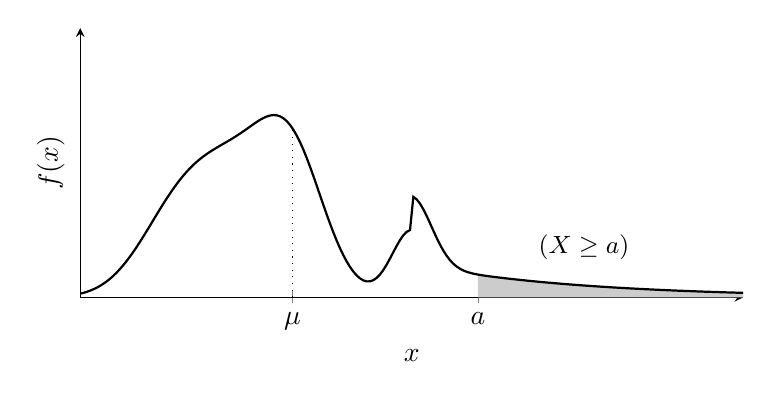
\begin{tikzpicture}
\begin{axis}[width=10cm,height=5cm,axis lines=left,xmin=0,xmax=10,ymin=0,ymax=0.32,xtick={3.2,6},xticklabels={$\mu$,$a$},ytick=\empty,xlabel={$x$},ylabel={$f(x)$},samples=200,domain=0:10]
\addplot[fill=gray!40,draw=none,domain=6:10] {0.1*exp(-0.5*((x-1.5)/0.6)^2)+0.15*exp(-0.5*((x-3.2)/0.5)^2)+0.12*exp(-0.5*((x-2.4)/0.6)^2)+0.08*exp(-0.5*((x-5)/0.3)^2)+0.04*exp(-(x-5)/2.5)*(x>5)} \closedcycle;
\addplot[black,thick] {0.1*exp(-0.5*((x-1.5)/0.6)^2)+0.15*exp(-0.5*((x-3.2)/0.5)^2)+0.12*exp(-0.5*((x-2.4)/0.6)^2)+0.08*exp(-0.5*((x-5)/0.3)^2)+0.04*exp(-(x-5)/2.5)*(x>5)};
\draw[dotted] (axis cs:3.2,0) -- (axis cs:3.2,0.2);
\node[font=\small] at (axis cs:7.6,0.06) {$\Prob(X\ge a)$};
\end{axis}
\end{tikzpicture}
\end{center}

\begin{note}
\notetitle \textbf{تعبیر:} اگر میانگین درآمد یک جامعه ۱۰ میلیون باشد، حداکثر $\frac1{5}$ مردم می‌توانند درآمد ۵۰ میلیون یا بیشتر داشته باشند؛ وگرنه میانگین از ۱۰ بیشتر می‌شد. مارکوف به هیچ اطلاعی جز نامنفی بودن و میانگین نیاز ندارد، و به همین دلیل معمولاً کران «شُلی» است. برای $a\le\E X$ کران بی‌اثر است (از ۱ بزرگ‌تر یا مساوی).
\end{note}

\subsection{نامساوی چبیشف \lr{(Chebyshev's Inequality)}}
\begin{theorem}[نامساوی چبیشف]
فرض کنید متغیر تصادفی $X$ دارای توزیعی با میانگین $\mu$ و واریانس $\sigma^2$ باشد. در این صورت، برای هر عدد حقیقی مثبت $k>0$ داریم:
\[
\boxed{\ \Prob\big(|X-\mu|\ge k\sigma\big)\le\frac{1}{k^2}\ }
\]
(معادلاً برای هر $\varepsilon>0$: $\Prob(|X-\mu|\ge\varepsilon)\le\frac{\sigma^2}{\varepsilon^2}$.)
\end{theorem}
\begin{proof}
متغیر نامنفی $Y=(X-\mu)^2$ را در نظر بگیرید که $\E Y=\sigma^2$. با نامساوی مارکوف روی $Y$ با $a=k^2\sigma^2$:
\[
\Prob(|X-\mu|\ge k\sigma)=\Prob\big((X-\mu)^2\ge k^2\sigma^2\big)\le\frac{\sigma^2}{k^2\sigma^2}=\frac1{k^2}.
\]
\end{proof}

\begin{center}
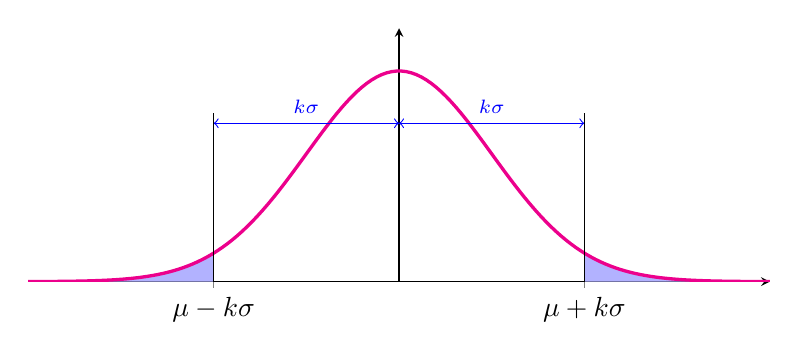
\begin{tikzpicture}
\begin{axis}[width=11cm,height=4.8cm,axis lines=middle,xmin=-4,xmax=4,ymin=0,ymax=0.48,xtick={-2,0,2},xticklabels={$\mu-k\sigma$,$\mu$,$\mu+k\sigma$},ytick=\empty,samples=150,domain=-4:4]
\addplot[fill=blue!30,draw=none,domain=-4:-2] {exp(-x^2/2)/sqrt(2*pi)} \closedcycle;
\addplot[fill=blue!30,draw=none,domain=2:4] {exp(-x^2/2)/sqrt(2*pi)} \closedcycle;
\addplot[magenta,very thick] {exp(-x^2/2)/sqrt(2*pi)};
\draw[<->,blue] (axis cs:-2,0.3) -- node[above,font=\scriptsize]{$k\sigma$} (axis cs:0,0.3);
\draw[<->,blue] (axis cs:0,0.3) -- node[above,font=\scriptsize]{$k\sigma$} (axis cs:2,0.3);
\draw (axis cs:-2,0) -- (axis cs:-2,0.32); \draw (axis cs:2,0) -- (axis cs:2,0.32);
\end{axis}
\end{tikzpicture}\\
{\small احتمال دو دُم (ناحیه آبی) برای \emph{هر} توزیعی حداکثر $1/k^2$ است.}
\end{center}

\begin{example}[مقایسه چبیشف با گاوسی]
برای $k=2$ و $k=3$ کران چبیشف را با مقدار دقیق برای توزیع گاوسی مقایسه کنید.
\begin{solution}
\begin{center}
\renewcommand{\arraystretch}{1.3}
\begin{tabular}{c|c|c}
$k$ & کران چبیشف $1/k^2$ & مقدار دقیق برای گاوسی\\\hline
$1$ & $1$ & $0.317$\\
$2$ & $0.25$ & $0.0455$\\
$3$ & $0.111$ & $0.0027$
\end{tabular}
\end{center}
کران چبیشف بسیار محافظه‌کارانه است، اما برای \emph{همه} توزیع‌ها با واریانس متناهی معتبر است. در واقع این کران قابل بهبود نیست: توزیعی وجود دارد که آن را به تساوی می‌رساند ($X=\pm k\sigma$ هر کدام با احتمال $\frac1{2k^2}$ و $X=0$ در بقیه موارد).
\end{solution}
\end{example}

\begin{theorem}[اثبات قانون ضعیف اعداد بزرگ]
اگر $X_1,X_2,\ldots$ \lr{i.i.d.} با میانگین $\mu$ و واریانس $\sigma^2<\infty$ باشند، آنگاه برای هر $\varepsilon>0$:
\[
\Prob\big(|\bar X_n-\mu|\ge\varepsilon\big)\le\frac{\sigma^2}{n\varepsilon^2}\ \xrightarrow{n\to\infty}\ 0 .
\]
\end{theorem}
\begin{proof}
$\E\bar X_n=\mu$ و $\Var\bar X_n=\frac{\sigma^2}{n}$ (جلسه دهم). نامساوی چبیشف را روی $\bar X_n$ اعمال کنید.
\end{proof}

\begin{example}[تعداد نمونه لازم]
برای تخمین احتمال $p$ یک رخداد با فرکانس نسبی در $n$ آزمایش مستقل، چند آزمایش لازم است تا با احتمال دست‌کم ۹۵٪ خطا از $0.05$ کمتر باشد؟
\begin{solution}
$\bar X_n$ میانگین $n$ برنولی با واریانس $\frac{p(1-p)}{n}\le\frac{1}{4n}$ است. با چبیشف:
$\Prob(|\bar X_n-p|\ge0.05)\le\frac{1}{4n(0.05)^2}=\frac{100}{n}\le0.05\Rightarrow n\ge2000$.
(با تقریب \lr{CLT} حدود $n\approx385$ کافی است: $1.96\cdot\frac{0.5}{\sqrt n}\le0.05$؛ چبیشف به دلیل کلی بودن، کران محافظه‌کارانه‌تری می‌دهد.)
\end{solution}
\end{example}

\section{آمار \lr{(Statistics)}}

\subsection{آمار در مقابل احتمال}
\begin{itemize}
\item \textcolor{red!70!black}{\textbf{احتمال:}} یک علم مجرد (\lr{abstract}) است که ابتدا تعدادی اصول موضوعه تعریف کرده و سپس بر پایه آنان اقدام به تعاریف جانبی و اثبات احکام می‌نماید.
\begin{itemize}
\item \textbf{اصول موضوعه:} فضای احتمال $(\Omega,\F,P)$ و اصول کولموگروف؛
\item \textbf{تعاریف جانبی:} احتمال شرطی، استقلال، متغیر تصادفی و \ldots؛
\item \textbf{احکام:} قانون بیز، قانون زنجیره‌ای، قضیه حد مرکزی، قانون اعداد بزرگ و \ldots
\end{itemize}
\item \textcolor{red!70!black}{\textbf{آمار:}} به کاربرد احتمال در حل مسائل دنیای واقع اطلاق می‌گردد، در شرایطی که اصول موضوعه فوق وجود خارجی نداشته و ناچار به «استدلال‌های استقرایی بر پایه مشاهدات» هستیم.
\item آمار در حالت کلی (به استثنای موارد خاص) علم کار کردن با مشاهدات و داده‌های واقعی است.
\end{itemize}

\begin{note}
\notetitle به بیان ساده: در \textbf{احتمال} مدل را می‌دانیم و درباره داده‌ها سؤال می‌کنیم (اگر سکه سالم باشد، احتمال ۷ شیر در ۱۰ پرتاب چقدر است؟). در \textbf{آمار} داده‌ها را داریم و درباره مدل سؤال می‌کنیم (۷ شیر در ۱۰ پرتاب دیده‌ایم؛ آیا سکه سالم است؟ احتمال شیر آن چقدر است؟). استدلال احتمالاتی «قیاسی» (از کل به جزء) و استدلال آماری «استقرایی» (از جزء به کل) است.
\end{note}

\subsection{توزیع‌های آماری \lr{(Statistical)} در مقابل تجربی \lr{(Empirical)}}
\begin{itemize}
\item مفاهیم (توزیع، میانگین و \ldots) \textbf{آماری} به مقادیر، توابع و یا سایر مفاهیم یقینی اطلاق می‌گردد که یک موجود تصادفی را توصیف می‌کنند. برای مثال متغیر تصادفی $X$، دارای توزیع آماری $f_X(x)$ و میانگین آماری $\E(X)$ است که خود یقینی (\lr{deterministic}) هستند.
\item مفاهیم \textbf{تجربی} به تقریب مابه‌ازای آماری خود از روی تعدادی مشاهدات اطلاق می‌گردند (مفاهیم تجربی بر خلاف مابه‌ازاهای آماری \textbf{ماهیت تصادفی} دارند).
\begin{itemize}
\item فرض کنید $X_1,X_2,\ldots,X_n$ نمونه‌های مستقل گرفته شده از متغیر تصادفی $X$ باشند.
\item توزیع انباشته تجربی $\hat F_X(x)$ و میانگین تجربی $\bar X_n$ به صورت زیر تعریف می‌شوند:
\[
\hat F_X(x)=\frac1n\sum_{i=1}^{n}\ind(X_i\le x),\qquad \bar X_n=\frac1n\sum_{i=1}^{n}X_i .
\]
\item مفاهیم تجربی فوق، خود متغیر تصادفی هستند (\textbf{چرا؟}). طبق قانون اعداد بزرگ، به ازای مقادیر بزرگ از $n$، مفاهیم تجربی (تحت شرایطی) به مابه‌ازاهای آماری خود میل می‌کنند.
\end{itemize}
\end{itemize}

\begin{question}[چرا مفاهیم تجربی، خود متغیر تصادفی هستند؟]
\begin{answer}
زیرا توابعی از نمونه‌های تصادفی $X_1,\ldots,X_n$ هستند. اگر آزمایش نمونه‌گیری را تکرار کنیم، نمونه‌های دیگری به دست می‌آید و در نتیجه $\bar X_n$ و $\hat F_X$ مقادیر دیگری خواهند داشت. در مقابل، $\E X$ و $F_X$ اعدادی ثابت‌اند که به نمونه‌ها بستگی ندارند.

\textbf{همگرایی:} برای هر $x$ ثابت، $\ind(X_i\le x)$ متغیرهای برنولی \lr{i.i.d.} با میانگین $F_X(x)$ هستند؛ پس $\hat F_X(x)$ میانگین نمونه‌ای آن‌هاست و طبق قانون اعداد بزرگ به $F_X(x)$ میل می‌کند (با $\E\hat F_X(x)=F_X(x)$ و $\Var\hat F_X(x)=\frac{F_X(x)(1-F_X(x))}{n}$). (قضیه گلیوِنکو--کانتلی حتی همگرایی یکنواخت روی همه $x$ را تضمین می‌کند.)
\end{answer}
\end{question}

\begin{center}
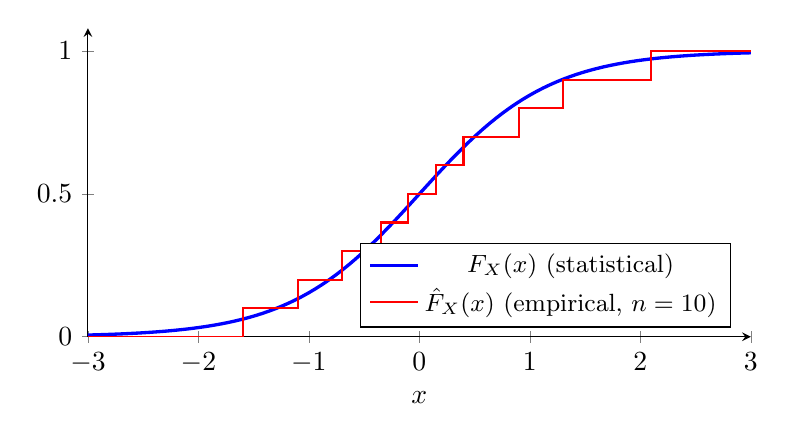
\begin{tikzpicture}
\begin{axis}[width=10cm,height=5.5cm,axis lines=left,xmin=-3,xmax=3,ymin=0,ymax=1.08,xlabel={$x$},legend pos=south east,legend style={font=\small},samples=100]
\addplot[blue,very thick,domain=-3:3] {1/(1+exp(-1.702*x))}; \addlegendentry{$F_X(x)$ \lr{(statistical)}}
\addplot[red,thick,const plot] coordinates {(-3,0) (-1.6,0) (-1.6,0.1) (-1.1,0.1) (-1.1,0.2) (-0.7,0.2) (-0.7,0.3) (-0.35,0.3) (-0.35,0.4) (-0.1,0.4) (-0.1,0.5) (0.15,0.5) (0.15,0.6) (0.4,0.6) (0.4,0.7) (0.9,0.7) (0.9,0.8) (1.3,0.8) (1.3,0.9) (2.1,0.9) (2.1,1) (3,1)}; \addlegendentry{$\hat F_X(x)$ \lr{(empirical, $n=10$)}}
\end{axis}
\end{tikzpicture}
\end{center}

\section{سرفصل‌های اصلی آمار}

\subsection{تخمین \lr{(Estimation)}}
متغیر تصادفی $X\sim f_X(x;\theta)$ را فرض نمایید، که در اینجا $\theta$ بیانگر یک یا چند پارامتر مربوط به توزیع باشند که \textcolor{red!70!black}{نامعلوم} هستند. فرض کنید که $n$ نمونه مستقل از $X$ به صورت $(X_1,X_2,\ldots,X_n)$ در دسترس باشند.
\begin{itemize}
\item \textbf{تخمین نقطه‌ای \lr{(Point Estimation)}:} به دست آوردن تخمینی \textcolor{red!70!black}{بهینه} از پارامتر $\theta$ به صورت $\hat\theta=\hat\theta(X_1,\ldots,X_n)$. (مثال: $\hat\mu=\bar X_n$ برای میانگین.)
\item \textbf{تخمین بازه‌ای \lr{(Interval Estimation)}:} فرض کنید $\theta$ یک‌بعدی باشد. هدف به دست آوردن بازه‌ای مانند $(\theta_l,\theta_u)$ است به طوری که $\Prob(\theta_l<\theta<\theta_u)\ge1-\delta$. (به این بازه «بازه اطمینان» با سطح $1-\delta$ می‌گویند؛ دقت کنید که $\theta_l,\theta_u$ توابعی از نمونه‌ها و در نتیجه تصادفی‌اند.)
\item \textbf{تخمین \lr{Bayesian}:} فرض کنید $\theta\sim f_\Theta(\cdot)$ یک متغیر تصادفی باشد. هدف به دست آوردن آماره‌های مرتبط با $\theta$ بعد از مشاهده نمونه‌هاست (یعنی توزیع پسین $f_{\Theta|X}$ با قانون بیز، مانند مثال سکه با احتمال نامعلوم در جلسه نهم).
\end{itemize}

\begin{note}
\notetitle مبحث تخمین بسیار گسترده بوده و اشکال غیرآماری نیز دارد. برای مثال، یکی از شکل‌های تخمین، تقریب مقدار یک متغیر تصادفی با استفاده از متغیرهای تصادفی وابسته به آن است (مثلاً تخمین $X$ از روی مشاهده $Y$). در اینجا، بر خلاف سناریوی شرح داده شده، توزیع مشترک تمام متغیرهای تصادفی دانسته فرض می‌شود. \textbf{تخمین میانگین مربع} (\lr{Mean Square Estimation}) از این جمله است و جلوتر مطرح خواهد گشت.
\end{note}

\begin{example}[تخمین بازه‌ای با \lr{CLT}]
از یک جامعه، ۱۰۰ نمونه گرفته‌ایم و میانگین نمونه‌ای $\bar X=50$ به دست آمده است. اگر بدانیم $\sigma=10$، یک بازه اطمینان ۹۵٪ برای $\mu$ بیابید.
\begin{solution}
طبق \lr{CLT}، $\bar X\approx\mathcal N(\mu,\frac{\sigma^2}{n})=\mathcal N(\mu,1)$. پس $\Prob(|\bar X-\mu|\le1.96)\approx0.95$، که معادل است با $\Prob(\bar X-1.96\le\mu\le\bar X+1.96)\approx0.95$. بازه: $[48.04,\ 51.96]$.
\end{solution}
\end{example}

\subsection{آزمون فرض \lr{(Hypothesis Testing)}}
متغیر تصادفی $X\sim f_X(x;\theta)$ با بردار پارامترهای نامعلوم $\theta$ را در نظر بگیرید. فرض کنید که $n$ نمونه مستقل از $X$ به صورت $(X_1,\ldots,X_n)$ در دسترس باشند.
\begin{itemize}
\item هدف پاسخ دادن به سؤالی در مورد پارامتر(های) $\theta$ است. برای مثال: آیا $\theta=\theta_0$ یا خیر؟
\item آزمون فرض کاربرد فراوانی در مطالعات آماری پزشکی و جامعه‌شناسی دارد (مثلاً: آیا یک داروی جدید اثری دارد یا تفاوت مشاهده‌شده تصادفی است؟).
\end{itemize}

\begin{example}[آیا سکه سالم است؟]
سکه‌ای را ۱۰۰ بار پرتاب کرده‌ایم و ۶۵ شیر آمده است. آیا می‌توان گفت سکه سالم است؟
\begin{solution}
فرض صفر $H_0$: $p=\frac12$. تحت $H_0$، تعداد شیرها $S\sim\mathrm{Bin}(100,\frac12)\approx\mathcal N(50,25)$. احتمال مشاهده نتیجه‌ای حداقل به این اندازه دور از ۵۰:
$\Prob(|S-50|\ge15)\approx2(1-\Phi(\frac{14.5}{5}))=2(1-\Phi(2.9))\approx0.004$. این احتمال (که «مقدار $p$» یا \lr{p-value} نام دارد) بسیار کوچک است؛ پس شواهد قوی علیه سالم بودن سکه داریم و $H_0$ را رد می‌کنیم. (مقایسه کنید با مثال جلسه سوم: انحراف ۱۰٪ از میانگین برای $n=100$ حدود ۳٫۵٪ احتمال داشت.)
\end{solution}
\end{example}

\subsection{پیش‌بینی \lr{(Prediction)}}
فرض کنید مدل تولید نمونه‌های تصادفی (منظور همان توزیع $f_X(x)$ است) معلوم است. در این صورت، هدف پیش‌بینی مقادیر تجربه مشاهدات آینده است:
\begin{itemize}
\item برای مثال، اگر اقدام به گرفتن $n$ نمونه به صورت \lr{i.i.d.} از $f_X(x)$ نماییم، توزیع میانگین تجربی $\bar X_n$ چه چیزی خواهد بود؟ (پاسخ تقریبی: $\mathcal N(\mu,\sigma^2/n)$ طبق \lr{CLT}.)
\item یا، در صورتی که احتمال موفقیت یک آزمایش مانند $A$ معلوم باشد، احتمال اینکه در $n$ بار انجام این آزمایش در آینده، تعداد آزمون‌های موفق چه توزیعی دارد؟ (پاسخ: $\mathrm{Bin}(n,\Prob(A))$.)
\end{itemize}

\section{بهینگی \lr{(Optimality)}}
\begin{itemize}
\item در بحث تخمین، بارها عبارت بهترین تخمین‌گر (یا \lr{Optimal Estimator}) شنیده خواهد شد. اما مقصود از \textbf{بهترین} چیست؟
\item \textcolor{red!70!black}{\textbf{بسیار مهم:}} تعریفی جهان‌شمول و یکتا برای بهترین وجود ندارد.
\item صفت بهترین، همواره با توجه به یک حیث (یا \lr{sense}) تعریف می‌شود. به عبارت صریح‌تر، یک معیار کمّی خطا/خوبی مانند $\ell(\theta,\hat\theta)$ را فرض نموده و سپس ادعا می‌کنیم تخمین‌گر $\hat\theta$ آن را کمینه/بیشینه می‌نماید.
\end{itemize}

\begin{example}[بهترین تخمین ثابت با معیارهای مختلف]
فرض کنید باید مقدار یک متغیر تصادفی $X$ را (بدون هیچ مشاهده‌ای) با یک عدد ثابت $c$ «پیش‌بینی» کنیم. بهترین $c$ چیست؟
\begin{solution}
\begin{itemize}
\item با معیار \textbf{خطای مربعی} $\ell=\E[(X-c)^2]$: $\E[(X-c)^2]=\Var X+(\E X-c)^2$ که در $c=\E X$ کمینه است. پس بهترین $c$ \textbf{میانگین} است.
\item با معیار \textbf{خطای مطلق} $\ell=\E|X-c|$: مشتق نسبت به $c$ برابر $\Prob(X<c)-\Prob(X>c)$ است که در \textbf{میانه} صفر می‌شود. پس بهترین $c$ میانه است.
\item با معیار \textbf{احتمال خطای صفر--یک} (برای متغیر گسسته) $\ell=\Prob(X\ne c)$: بهترین $c$ \textbf{مُد} است.
\end{itemize}
این مثال به‌روشنی نشان می‌دهد که «بهترین» بدون مشخص کردن معیار معنا ندارد؛ و سه آماره جلسه دهم (میانگین، میانه، مد) هر کدام تحت یک معیار بهینه‌اند.
\end{solution}
\end{example}

\section{تمرین‌های تکمیلی}

\begin{exercise}
تعداد درخواست‌های روزانه یک سایت به طور متوسط ۱۰۰۰ است. (الف) با مارکوف، کرانی برای احتمال بیش از ۲۰۰۰ درخواست بیابید. (ب) اگر انحراف معیار ۱۰۰ باشد، با چبیشف کران بهتری بیابید.
\end{exercise}
\begin{solution}
(الف) $\Prob(X\ge2000)\le\frac{1000}{2000}=0.5$.
(ب) $\Prob(X\ge2000)\le\Prob(|X-1000|\ge1000)\le\frac{100^2}{1000^2}=0.01$. دانستن واریانس، کران را ۵۰ برابر بهتر کرد.
\end{solution}

\begin{exercise}
نشان دهید برای هر متغیر تصادفی با میانگین $\mu$ و واریانس $\sigma^2$، دست‌کم ۷۵٪ احتمال در بازه $[\mu-2\sigma,\mu+2\sigma]$ قرار دارد.
\end{exercise}
\begin{solution}
با چبیشف و $k=2$: $\Prob(|X-\mu|<2\sigma)\ge1-\frac14=0.75$.
\end{solution}

\begin{exercise}
با استفاده از نامساوی مارکوف روی $e^{tX}$، نشان دهید برای هر $t>0$: $\Prob(X\ge a)\le e^{-ta}M_X(t)$ (کران چرنوف). سپس برای $X\sim\mathcal N(0,1)$ بهترین کران را بیابید.
\end{exercise}
\begin{solution}
چون $e^{tX}$ نامنفی و $x\mapsto e^{tx}$ صعودی است: $\Prob(X\ge a)=\Prob(e^{tX}\ge e^{ta})\le\frac{\E e^{tX}}{e^{ta}}$.
برای گاوسی استاندارد: $e^{-ta+t^2/2}$ که در $t=a$ کمینه می‌شود: $\Prob(X\ge a)\le e^{-a^2/2}$. این کران نمایی (برخلاف چبیشف که $\frac{1}{a^2}$ است) رفتار واقعی دم گاوسی را به خوبی نشان می‌دهد.
\end{solution}
